\documentclass[10pt,landscape]{article}
% \pagestyle{headings}
\usepackage{multicol}
\usepackage[landscape]{geometry} 
\usepackage{amsfonts}
\usepackage{amssymb}
\usepackage{amsmath}
\usepackage{latexsym}
\usepackage{enumerate}
\usepackage{verbatim}
\usepackage{multirow}
\usepackage[lofdepth,lotdepth]{subfig}
\usepackage[pdftex]{graphicx}
\setlength{\parindent}{0pt}
\setlength{\parskip}{0pt plus 0.5ex}
% \setlength{\parskip}{1ex plus 0.5ex minus 0.2ex}
\setlength{\topmargin}{-1.35in}
\setlength{\textheight}{8in}
\setlength{\oddsidemargin}{-0.75in}
\setlength{\evensidemargin}{-0.75in}
\setlength{\textwidth}{10.5in}
% \setlength{\baselineskip}{-1pt}
% \renewcommand{\baselinestretch}{0.5}

\makeatletter
\renewcommand{\section}{\@startsection{section}{1}{0mm}%
  {-1ex plus -.5ex minus -.2ex}%
  {0.5ex plus .2ex}%x
  {\normalfont\large\bfseries}}
\renewcommand{\subsection}{\@startsection{subsection}{2}{0mm}%
  {-1explus -.5ex minus -.2ex}%
  {0.5ex plus .2ex}%
  {\normalfont\normalsize\bfseries}}
\renewcommand{\subsubsection}{\@startsection{subsubsection}{3}{0mm}%
  {-1ex plus -.5ex minus -.2ex}%
  {1ex plus .2ex}%
  {\normalfont\small\bfseries}}
\renewcommand{\thesection}{\Roman{section}}
\makeatother

\newcommand{\ps}{\ \vspace{0.05in}}
\newcommand{\dg}{$^\circ$ }
\newcommand{\img}[1]{\includegraphics[scale=0.5]{#1}}

% Don't print subsection numbers
\setcounter{secnumdepth}{1}

\thispagestyle{empty} 

\begin{document}

\raggedright
\begin{multicols*}{3}
  
  \section*{Synthesis In Brief - Feynman Liang\\
    CHEM231 - Spring 2012\\
    Amherst College}
  
  \begin{scriptsize}

    \section{Designing Syntheses}

    \subsection{Consider the target's:}

    \begin{itemize}
    \item Molecular size/density
    \item Number of stereocenters
    \item Elements present
    \item Functional groups present
    \item Chemical reactivity
    \end{itemize}

    \subsection{Synthesis Considerations}

    \begin{itemize}
    \item Must be selective to be useful (protecting groups, solvent choice)
    \item Other functional groups on the molecule
    \item Be aware of limitations of proposed transformations
    \end{itemize}

    \subsection{Retrosynthesis}
    Basically disconnect groups one by one and work backwards from target to start.
    
    \section{Common retrosynthetic patterns}

    \subsection{Carbonyl patterns}
    
    \begin{itemize}
    \item Methyl ketones with alkyl groups attached to $\alpha$-carbon\\
      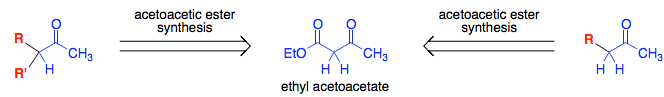
\includegraphics[scale=0.35]{ace-est.png}
    \item Carboxylic acid with alkyl groups attached to $\alpha$-carbon\\
      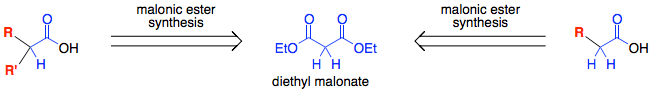
\includegraphics[scale=0.35]{mal-est.png}
    \item $\beta$-hydroxy carbonyl\\
      \img{aldol.png}
    \item $\alpha,\beta$-unsaturated aldehyde/ketone: E1cb (removal of $\alpha$-proton
      followed by elimination of $\beta$-hydroxy with - charge)
      \img{aldol2.png}
    \end{itemize}

    \subsection{Dicarbonyl patterns}
    
    \begin{itemize}
    \item 1,3-dicarbonyl\\
      \img{claisen1.png}\\
      \img{alkylation1.png}
    \item 1,3-$\beta$-ketoester\\
      \img{claisen2.png}
    \item 1,5-dicarbonyl\\
      \img{michael1.png}
    \end{itemize}

    \subsection{Enolate patterns}

    \begin{itemize}
    \item Non-methyl ketone\\
      \img{culi1.png}
    \item Non-methyl ketone (branching at $\alpha$)\\
      \img{alkylation2.png}
    \item Non-methyl ketone (branching at $\beta$)\\
      \img{culi2.png}
    \end{itemize}
    
    \subsection{Unconjugated alkenes}
    
    \img{wittig1.png}

    \subsection{Alcohol patterns}

    \begin{itemize}
    \item Tertiary alcohol\\
      \img{mgx1.png}
      \img{mgx2.png}
      \img{hg-red1.png}
    \item Secondary alcohol\\
      \img{mgx3.png}
      \img{hydry-1.png}
      \img{hg-red2.png}
      \img{bh3-1.png}
    \item Primary alcohol\\
      \img{mgx4.png}
      \img{hydry-2.png}
      \img{bh3-2.png}
    \end{itemize}
    
    \subsection{EAS}

    \begin{itemize}
    \item Must proceed through \textbf{privileged systems}:
      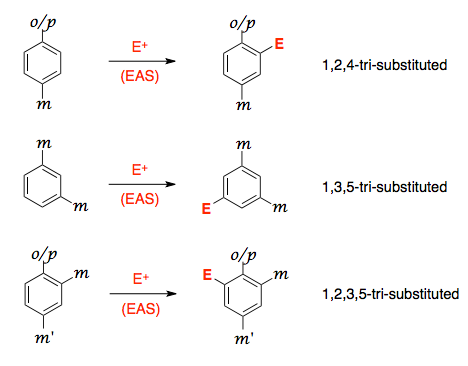
\includegraphics[scale=0.4]{privsys.png}
    \item \textbf{EAS Rules:}
      \begin{itemize}
      \item Can stop each EAS after one reaction
      \item Only o/p di-substituted isomers can be seperates (no tri/tetra separation)
      \item Proceed only through \textbf{privileged systems}: substituents symmetric or all direct
        to same positions
      \item No Friedel Crafts alkyl/acylation (alkyl and acyl halide rxn through carbocation/acylium
        intermediate) if R-NO$_2$ present (too deactivating)
      \item No Friedel Crafts alkylation (alkyl halide rxn through carbocation) if
        carbocation rearrangements are possible
      \end{itemize}
    \item Strategies:
      \begin{itemize}
      \item \textbf{Sulfonation/sulfonation is reversible}, can block 5 position of 1,2,3-trisub
      \item NO$_2$ directs m, reduction (and Sandmeyer) converts to o/p director NH$_2$
        (or from Sandmeyer: OH, Cl, Br, I)
      \item Alkyl directs o/p, converted to acyl via \textbf{KMnO$_4$ oxidation }
      \item Acyl directs m, can be converted to corresponding alkyl via \textbf{Clemmenson
          reduction}
      \end{itemize}
    \end{itemize}

    \section{Ground Rules for Synthesis}

    \begin{itemize}
    \item Any inorganic starting materials
    \item Any organometallic reagent (RMgX or R$_2$CuLi) where R=
      \begin{enumerate}[a)]
      \item Allyl group
      \item Phenyl ring
      \item Saturated alkyl chain with $\leq$4 carbons
      \end{enumerate}
    \item Organic reagents:
      \begin{enumerate}[a)]
      \item Any saturated alcohol, aldehyde, ketone, carboxylic acid, alkyl halide with
        $\leq$4 carbons
      \item Any ylide with $\leq$4 carbons (phenyls in PPh$_3$ don't count)
      \item Any ester which acid component contains $\leq$4 carbons (don't count ester's
        carbons)
      \end{enumerate}
    \item ONLY ONE functional group per molecule. ex. no Michael acceptors b/c contains
      both alkene and carbonyl, no vinyl halides (allyl permitted)
    \end{itemize}  

    \subsection{ Allowed reagents:}
    
    \begin{itemize}
    \item \textbf{Diethyl carbonate} - starting ester (to make
      diesters from ketones)\\
      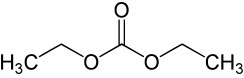
\includegraphics[scale=0.25]{allowed/diethylcarbonate.jpg}
    \item Ethyl acetoacetate - acetoacetic ester synthesis\\
      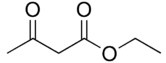
\includegraphics[scale=0.25]{allowed/ethylacetoacetate.jpg}
    \item \textbf{Diethyl malonate} - malonic ester synthesis\\
      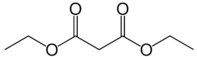
\includegraphics[scale=0.25]{allowed/diethylmalonate.jpg}
    \item 1,2-ethanediol - carbonyl protecting group\\
      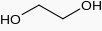
\includegraphics[scale=0.25]{allowed/1,2-ethanediol.jpg}
    \item \textbf{Diethyl oxalate} - only 1,2-dicarbonyl, not too sure... 
      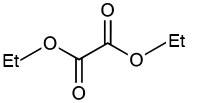
\includegraphics[scale=0.25]{allowed/diethyloxalate.jpg}
    \item \textbf{Allyl bromide} - substitution/alkene\\
      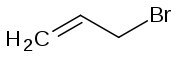
\includegraphics[scale=0.25]{allowed/allylbr.jpg}
    \item \textbf{Benzyl bromide} - substitution\\
      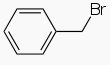
\includegraphics[scale=0.25]{allowed/benzylbr.jpg}
    \item \textbf{Cyclohexanone} - ketone, 6-ring\\
      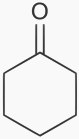
\includegraphics[scale=0.25]{allowed/cyclohexanone.jpg}
    \item \textbf{Cycloopentanone} - ketone, 5-ring\\
      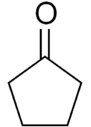
\includegraphics[scale=0.25]{allowed/cyclopentanone.jpg}
    \item \textbf{Tosyl Chloride} - TsCl, alcohols $\rightarrow$ R-OTs\\
      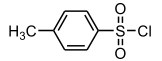
\includegraphics[scale=0.25]{allowed/TsCl.jpg}
    \item \textbf{Pyridine} - weak base/proton sink\\
      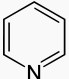
\includegraphics[scale=0.25]{allowed/pyridine.jpg}
    \item \textbf{mCPBA} - epoxidation rxn agent\\
      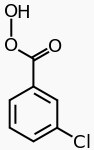
\includegraphics[scale=0.25]{allowed/mCPBA.jpg}
    \item \textbf{Dimethyl sulfide} - ozonolysis reducing agent\\
      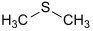
\includegraphics[scale=0.25]{allowed/dimethylS.jpg}
    \item \textbf{Mercuric acetate} - oxymercuration rxn agent\\
      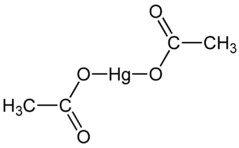
\includegraphics[scale=0.25]{allowed/hgoac2.jpg}
    \item \textbf{Bromobenzene} - EAS\\
      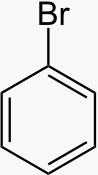
\includegraphics[scale=0.25]{allowed/bromobenzene.jpg}
    \item \textbf{Benzaldehyde} - EAS\\
      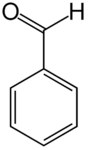
\includegraphics[scale=0.25]{allowed/benzaldehyde.jpg}
    \item \textbf{Benzoic acid} - EAS\\
      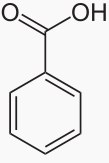
\includegraphics[scale=0.25]{allowed/benzoicacid.jpg}
    \item \textbf{Benzene} - EAS\\
      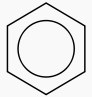
\includegraphics[scale=0.25]{allowed/benzene.jpg}
    \item \textbf{Toluene} - EAS\\
      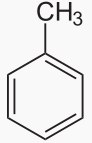
\includegraphics[scale=0.25]{allowed/toluene.jpg}
    \end{itemize}
  \end{scriptsize}
\end{multicols*}
\end{document}
%%% Local Variables: 
%%% mode: latex
%%% TeX-master: t
%%% End: 
